\documentclass[11pt,a4paper]{article}

\usepackage[polish]{babel}
\usepackage{polski}
\usepackage[utf8]{inputenc}
\usepackage[T1]{fontenc}
\usepackage{graphicx}
\usepackage{color}
\usepackage{placeins}
\usepackage[math]{anttor}
\usepackage{natbib}
\usepackage{url}
\usepackage{float}
\usepackage[font=small,labelfont=bf]{caption}
\usepackage{array}
\frenchspacing

\newcommand{\todo}[1]{\colorbox{yellow}{#1}}

\begin{document}

\title{Automatyczna klasyfikacja i ekstrakcja tematu krótkich notatek w języku polskim}
\author{Paweł Obrok\\pod kierunkiem dr. Michała Korzyckiego}

\maketitle
\pagebreak

\todo{Oświadczenie prawnoautorskie}
\pagebreak

\todo{Strona tytułowa po angielsku}
\pagebreak

\tableofcontents
\pagebreak

\section{Wstęp}
\section{Terminy i oznaczenia}

\begin{itemize}
\item $df_i$ (Document Frequency) --- liczba dokumentów zawierjących $i$-ty token
\item $gf_i$ (Global Frequency) --- stosunek liczby wystąpień $i$-tego tokenu do liczby wszystkich wyrazów w korpusie
\item $tf_i^j$ (Term Frequency) --- stosunek liczby wystąpień $i$-tego tokenu do liczby wszystkich wyrazów w $j$-tym dokumencie
\item Dokument --- tekst lub fragment tekstu
\item FN (False Negatives) --- liczba odrzuconych dokumentów skojarzonych
\item FP (False Positives) --- liczba zwróconych dokumentów skojarzonych
\item Korpus --- zbiór dokumentów
\item LDA --- Latent Dirichlet Allocation
\item LSI --- Latent Semantic Indexing
\item Leksykon --- zbiór wszystkich tokenów występujących w korpusie
\item Przeuczenie --- zjawisko polegające na zbyt dokładnym odwzorowaniu danych treningowych przez model i utracie zdolności uogólniania
\item Schemat Wagowy --- sposób w jaki dokument jest transformowany do reprezentacji wektorowej
\item Skojarzony --- (o dokumencie) zgodny z kryteriami wyszukiwania, uznany za podobny do dokumentu wzorcowego
\item TN (True Negatives) --- liczba odrzuconych dokumentów nieskojarzonych
\item TP (True Positives) --- liczba zwróconych dokumentów skojarzonych
\item Token --- wyraz, znak interpunkcyjny lub grupa znaków traktowana jako całość (na przykład liczba)
\item VSM (Vector Space Model) --- modelowanie języka przez przedstawianie dokumetów jako wektorów
\end{itemize}

\pagebreak

\section{Podstawy teoretyczne}

W tym rozdziale opisana jest ogólnie koncepcja wektorowego modelowania
dokumentów oraz metody, które poddano porównaniu w tej pracy, a które od tej
koncepcji pochodzą. W dalszej części rozdziału zawarto opis metryk perpexity,
dokładności i kompletności wykorzystywanych przy ocenie działania modeli
językowych i systemów wyszukiwania informacji.

\subsection{Vector Space Model}

\label{weighting-theory} Model przestrzeni wektorowej (Vector Space Model -
VSM) to metoda modelowania języka polegająca na reprezentowaniu dokumentów jako
wekorów co umożliwia na przykład porównywanie ich metodami algebry liniowej.
Wektor dla $i$-tego dokumentu ma postać:

\begin{equation}
d_i = (w^i_0, w^i_1, \ldots, w^i_N)
\end{equation}

gdzie wymiar $w^i_k$ odpowiada $k$-temu tokenowi z leksykonu. Współczynniki te
nazywane są także wagami i mają oddawać znaczenie danego tokenu w danym
dokumencie --- powinny być tym wyższe im bardziej kluczowy dla sensu $i$-tego
dokumentu jest $k$-ty token. Przyjmuje się zwykle, że wymiary odpowiadające
tokenom nie występującym w danym dokumencie są zerowe.

Najbardziej ogólnie wagi $w^i_k$ uzyskuje się przez pomnożenie wagi globalnej
$g_k$, która ma odzwierciedlać popularność tokenu w całym korpusie i wagi
lokalnej $l^i_k$, która opisuje stricte znaczenie tokenu w danym dokumencie.
Tabele \ref{global-weights} i \ref{local-weights} podsumowują popularnie
stosowane wagi globalne i lokalne. Ich drobiazgowe porównanie dla języka
polskiego znaleźć można w \cite{figiel}. Dobór tych dwóch wag nazywamy
schematem wagowym.

\begin{table}[h]
\caption{Możliwe wagi globalne $g_k$}
\label{global-weights}
\begin{tabular}[c]{|c|p{0.7\linewidth}|}
\hline
$1$ & Brak wagi globalnej --- częstość występowania tokenów w całym korpusie jest ignorowana \\\hline
$\frac{1}{\sum_j (l^j_k)^2}$ & Normalizacja --- tutaj przez sumę kwadratów wag lokalnych tokenu w całym korpusie\\\hline
$\frac{gf_k}{df_k}$ & gf-idf --- waga tym większa im więcej razy występuje dany token i tym mniejsza im więcej dokumentów go zawiera\\\hline
$log(\frac{n}{df_k}) + 1$ & idf --- logarytm z liczby dokumentów w których występuje dany token znormalizowanej przez liczbę wszystkich dokumentów\\\hline
$1 - \sum_{i/0}^n \frac{tf^i_klog(tf^i_k)}{log(n)}$ & Entropia --- waga pochodząca z teorii informacji, ilość informacji którą daje pojawienie się danego tokenu o numerze tekstu, w którym to nastąpiło\\\hline
\end{tabular}
\end{table}

\begin{table}[h]
\caption{Możliwe wagi lokalne $l^i_k$}
\label{local-weights}
\begin{tabular}[c]{|c|p{0.875\linewidth}|}
\hline
$1$ & Waga binarna --- zachowana zostaje jedynie informacja o fakcie wystąpienia tokenu, liczba wystąpień jest ignorowana\\\hline
$t^i_k$ & Częstość występowania --- najprostsza waga, można powiedzieć, że inne są próbą jej usprawnienia przez odpowiednid wygładzenie\\\hline
$\sqrt{t^i_k}$ & Wygładzona częstość występowania --- aby oddać fakt, kolejne wystąpienia tego samego wyrazu dają stosunkowo mniejszą wskazówkę co do jego znaczenia dla danego dokumentu można wygładzić częstość występowania pierwiatskiem lub logarytmem\\\hline
\end{tabular}
\end{table}

Konkretny schemat wagowy dobiera się empirycznie, często pod jakąś klasę
problemów. Dla zadań typu information retrieval dobrze sprawdzają się lokalne
wagi wygładzone i entropia jako waga globalna z czego można wywnioskować, że
obserwacja o mniejszym znaczeniu kolejnych wystąpień tokenu w tym samym
dokumencie jest trafna.

Brak wagi globalnej daje z reguły znacznie gorsze wyniki niż pozostałe
możliwości. Jej zastosowanie pozwala automatycznie wykryć wyrazy takie jak
spójniki, które występują bardzo często we wszystkich tekstach, a nie mają
dużego ładunku semantycznego. W korpusach dotyczących jednej dziedziny mogą się
pojawić inne wyrazy o takiej charakterystyce, przykładowo wyraz ,,wyraz''
występuje bardzo często w tej pracy i najprawdopodobniej nie niesie wiele
informacji o tematyce poszczególnych jej akapitów, w których się pojawia.

Podobnie zastosowanie binarnej wagi lokalnej negatywnie wpływa na jakość
otrzymywanych wyników. Utrata informacji na temat dokumentu jest w tym wypadku
zbyt duża, dodatkowe wystąpienia tokenu mimo iż nie tak znaczące jak pierwsze
są jednak wskazówką co do większego znaczenia tego tokenu w tekście.

\FloatBarrier

\subsection{Latent Semantic Indexing}
\subsection{Latent Dirichlet Allocation}
\label{sec:lda}

Podczas gdy LSI ma u swoich podstaw metodę algebraiczną redukcji wymiarowości
macierzy przy utracie jak najmniejszej ilości zawartej w tej macierzy
informacji intuicja stojąca za LDA jest znacznie bliżej spokrewniona z
wyobrażeniami na temat powstawania dokumentów tekstowych. Jak zostanie jednak
przedstawione w tym rozdziale ostatecznie LDA również sprowadza się do redukcji
wymiaru macierzy term-dokument przez wprowadzenie nowej przestrzeni, w której
reprezentowane będą dokumenty.

\subsubsection{Intuicja}

LDA to probabilistyczny model generatywny opisujący powstawanie dokumentów.
Zakłada, że dokumenty są zbiorami wyrazów i kolejność ich występowania nie ma
znaczenia. Zakłada następnie, że każdy dokument traktuje o małej liczbie
tematów z pewnego zbioru tematów, których liczba jest znana \emph{a priori}.

\todo{Moar here}

\subsubsection{Dobierani parametrów modelu}

\subsection{Perplexity}

Współczynnik perplexity, który zaproponowany został do oceny modeli języka
\cite{bahl-perplexity}, ma oddawać niejako poziom ''zaskoczenia'' niewidzianymi
dotąd danymi. Dla rozkładu prawdopodobieństwa $p$ definiujemy go jako
eksponentę entropii $p$, czyli:

\begin{equation}
  \label{perplexity-definition}
  2^{H(p)} = 2^{-\sum_x p(x)log_2 p(x)}
\end{equation}

Dla dyskretnej dystrybucji o $n$ równoprawdopodonych możliwych wydarzeniach
współczynnik perplexity wyniesie $n$ --- daje to możliwość porównania innego
rodzaju dytrybucji (rónież ciągłych --- zamieniwszy sumę we wzorze
\ref{perplexity-definition} na całkę) pod względem ich ,,rozstrzelenia'', a co
więcej daje dodatkową intuicję, że dana dystrybucja będzie generować dane,
które będą podobnie ,,zaskakujące'' jak rzut $n$-ścienną kostką.

Jeżli chcemy wykorzystać perplexity do oceny modelu jakiegoś zjawiska $q$,
który przypisuje zdarzeniom prawdopodobieństwa $q(x)$, to możemy obliczyć
znormalizowany współczynnik perplexity dla pewnego zbioru obserwacji tego zjawiska
$\{x_1, x_2, \ldots, x_N\}$ następująco:

\begin{equation}
  2^{H(q)} = 2^{-\frac{1}{N}\sum_i^N log_2 p(x_i)}
\end{equation}

Zaletą tego podejścia jest możliwość całkowicie automatycznej oceny jakości
modelu --- modele lepiej opisujące dane zjawisko będą przyporządkowywać wyższe
prawdopodobieństwa wydarzeniom, które rzeczywiście zachodzą i co za tym idzie
będą miały niższy współczynnik perplexity. Zwykle taka ewaluacja stosowana jest
do upewnienia się, że model nie jest przeuczony, że jest w stanie uogólniać
swoje przewidywania na sytuacje inne niż dane treningowe. W takim wypadku
alalizuje się współczynnik perplexity obliczony dla dodatkowego zbioru
danych, które nie były wykorzystane do treningu i przykładowo zatrzymuje
interacyjny proces uczenia modelu, kiedy zaczyna on wzrastać.

W modelach języka jako pojedyncze zdarzenia stosuje się wyrazy lub zdania.
Przykładowo \cite{perplexity-estimate} podaje współczynnik perplexity 247 dla
korpusu Browna, zawierającego zróżnicowane teksty w języku algielskim
osiągnięty przez model trigramowy. Jest to równoważne przypadkowi, gdy każde
słowo jest wybierane niezależnie z równym prawdopodobieństwem spośród 247
możliwości.

\subsection{Dokładność i kompletność}

\todo{Citation?}

Aby ocenić i porównywać wyniki działania algorytmów wyszukujących dokumenty w
korpusach należy wprowadzić formalne metryki opsisujące jakość wyników przez
nie uzyskiwanych. Należy przy tym zauważyć, że znaczenie ma nie tylko fakt
zwrócenia wielu czy nawet wszystkich dokumentów skojarzonych z zapytaniem, ale
także liczba zwróconych dokumentów nieskojarzonych, gdyż stanowią one szum i
wyniki zaweierające wiele takich dokumentów wymagają dalszego, ręcznego
przetwarzania. Aby uchwycić te dwie interesujące nas cechy stosuje się
zazwyczaj dwie metryki: dokładność i kompletność.

Kompletność ma wyrażać jak dużo interesujących wyników zostało odnalezione przez
algorytm, obliczana jest według wzoru:

\begin{equation}
  K = \frac{TP}{TP + FN}
\end{equation}

W tym wzorze licznik, to liczba poprawnie zwrócocnych dokumentów, a mianownik
to po prostu liczba wszyskich dokumentów skojarzonych, które występują w danym
korpusie.

Dokładność opisuje udział skojarzonych dokumentów w zwróconych wynikach, formalnie
opisuje ją wzór:

\begin{equation}
  D = \frac{TP}{TP + FP}
\end{equation}

Te dwie metryki stoją do siebie w pewnym sensie w opozycji --- w wielu
systemach możliwe jest sterowanie progiem detekcji i zwiększenie kompletności
kosztem dokładności lub odwrotnie. Z tego też powodu analizuje się je zwykle w
tandemie i interesujące są nie tyle ich wartości jako takie, co zależność
między nimi.

\section{Architektura rozwiązania}

W tym rozdziale zawarty został szczegółowy opis rozwiązań użytych w tej pracy.
Pierwsza część omawia sposób przetwarzania danych wejściowych (zbioru
dokumentów, patrz \ref{data-description}), druga natomiast omawia po krótce
wykorzystane w badaniach biblioteki programistyczne.

\subsection{Procedura przetwarzania}

\todo{This is most likely not complete}

Poniżej znajduje się omówienie krok po kroku sposobu w jaki osiągnięto
prezentowane wyniki. Omawiane są zarówno operacje wykonywane na danych, wybór
konkretnych możliwości w takich kwestiach jak schemat wagowy (patrz
\ref{weighting-theory}), jak i sposób obliczania metryk jakości rozwiązania:
wpółczynnika perplexity oraz współczynnika $M$ opisującego
jakość zwróconego rankingu dokumentów.

\subsubsection{Sprowadzenie do form podstawowych}

Metody macierzowe zachowują się znacznie lepiej dla mniejszych rozmiarów
leksykonu, a co za tym idzie mniejszych rozmiarów wektorowej reprezentacji
dokumentów. Poza oczywistym zyskiem polegającym na krótszym czasie
przetwarzania pomniejszenie leksykonu w stosunku do liczby i długości
dokumentów sprawia także, że metody te mogą łatwiej wykrywać, które wyrazy są
powiązane --- każdy wyraz występuje w większej liczbie kontekstów, umożliwiając
zebrania na jego temat więcej informacji.

W tym wypadku zastosowano słownik fleksyjny (patrz \ref{sec:clp}) do
sprowadzenia wyrazów występujących w tekście do form podstawowych --- ta
operacja nie tylko zmniejsza liczbę różnych tokenów, ale także umożliwia na
dalszych etapach rozpoznanie faktu, że kilka różnych form jest w istocie tym
samym wyrazem. Bez niej przykładowo wyrazy ,,bliźniak`` i ,,bliźniaka`` byłyby
traktowane jako całkowicie różne i nie wnosiły by nic do oceny przez algorytm
tekstów, w których występują.

W \cite{manning-schuetze} sugerowano, że tego typu krok można pominąc posiadając
odpowiednio duży korpus danych, jednak uwaga ta dotyczy języka angielskiego, w
którym liczba form wyrazów jest stosunkowo mała. Polski jako język silnie
fleksyjny wymagałby w tym wypadku zapewne zbioru danych o dużo więksych
rozmiarach, którego przetwarzanie mogłoby być niepraktyczne.

\subsubsection{Preprocessing}

Aby zmniejszyć rozmiar przetwarzanych danych i poprawić ich uwarukowanie po
sprowadzeniu wszystkich wyrazów danego dokumentu do form podstawowych
zastosowano dodatkowy preprocessing polegający na odrzuceniu wyrazów
występujących w więcej niż 70\% dokumentów i takich, które wystąpiły w co
najwyżej jednym dokumencie. Te pierwsze nie niosą żadnej informacji o rodzaju
tekstu, w którym występują ze względu na swoją pospolitość. Powiązania tych
drugich nie mogłyby być wychwycone przez algorytmy redukcji wymiaru macierzy.

Zastosowano również kilka innych prostych operacji, jak na przykład
zamienienie wszystkich liczb na token ''NUMBER'' a wyrażeń typ ''2:3''
na token ''RATIO''.

Przykładowo następujący dokument:

\begin{quote}
\#000064\\
Drużyna Krzysztofa Oliwy - New Jersey Devils, mająca najlepszy
bilans w całej NHL, odniosła kolejne zwycięstwo, pokonując w
środę na własnym lodowisku New York Rangers 4:1.
\end{quote}

po poddaniu preprocessingowi przyjmie postać:

\begin{quote}
NUMBER\\
drużyna Krzysztof oliwa - new jersey devils , mający najlepszy bilans
cały NHL , odnieść kolejny zwycięstwo , pokonując środa własny lodowisko new
York rangers RATIO
\end{quote}

\subsubsection{Dobór schematu wagowego}
\label{weighting}

Bezpośrednie zastosowanie podejścia bag-of-words może dawać mylny obraz
dokumentu --- pewne wyrazy mogą pojawiać się bardzo często a mimo to nie
dostarczać żadnej pożytecznej informacji o danym dokumencie ze względu na fakt
występowania bardzo często w danym korpusie. Innym problemem może być
przecenianie wielokrotnego występowania danego wyrazu --- trzykrotne pojawienie
się pewnego wyrazu raczej nie sugeruje trzykrotnie większego prawdopodobieństa,
że jest on kluczowy dla tekstu. Aby rozwiązać pierwszy z tych problemów stosuje
się normalizowanie wag wyrazów w danym dokumencie przez jakiś współczynnik
charakteryzujący częstość występowania tego wyrazu w całym korpusie. Drugi z
nich można rozwiązać przez zastosowanie funkcji typu logarytm czy pierwiastek.
Dokładny dobór zastosowanych na tym etapie przekształceń nazywamy schematem
wagowym.

W tej pracy zastosowano schemat wagowy nazywany ''Log Entropy''.  Intuicyjnie
polega on na wykorzystaniu ilości informacji w sensie Shannona niesionej przez
dany wyraz jako czynnika normalizacyjnego (dla często spotykanych wyrazów
będzie on niski) i zastosowaniu logarytmu jako funkcji wygładzającej.

Mając daną macierz $w_{ij}$, której $j$-ty wiersz odpowiada $j$-temu
dokumentowi, a jego $i$-ta pozycja zawiera liczbę wystąpień $i$-tego wyrazu w
tym dokumecie dokonujemy przeształcenia opisanego równaniami
\ref{eq:log-entr-beg}--\ref{eq:log-entr-end} uzyskując macierz $a_{ij}$
zawierającą nowe wagi wyrazów.

\begin{equation}
  \label{eq:log-entr-beg}
  p_{ij} = \frac{tf_{ij}}{gf_i}
\end{equation}

\begin{equation}
  g_i = 1 + \sum_{j=1}^n \frac{p_{ij} log(p_{ij})}{log(n)}
  \todo{$log(p_{ij}) = -\infty?$}
\end{equation}

\begin{equation}
  \label{eq:log-entr-end}
  a_{ij} = g_i log(tf_{ij} + 1)
\end{equation}

Drobiazgowe omówienie i porównanie różnych schematów wagowych znaleźć moż\-na w
\cite{figiel}.

\subsubsection{Przetwarzanie zapytania}
\label{processing}

Mając dany model macierzowy dla pewnego korpusu pojawia się standardowy problem
wykonania zapytania do modelu i uzyskania z niego informacji. Dla pewnego
dokumentu stanowiącego zapytanie $d_q$ (może to być dokument, podobny do tych,
które znajdują się w korpusie, albo po prostu zbitek wyrazów w rodzaju zapytań
wprowadzanych zwykle w wyszukiwarce internetowej) chcielibyśmy uzyskać teksty z
korpusu $d_i$ posortowane według malejącej oceny podobieństwa tych tekstów do
$d_q$. W tym celu obliczamy dla każdego $d_i$ ranking $r_i$ według wzorów
\ref{similarity-computation-beg}-\ref{similarity-computation-end}.

\begin{equation}
\label{similarity-computation-beg}
  \langle d_i, d_j \rangle = \sum_k^n d_{ik}d_{jk}
\end{equation}

\begin{equation}
  ||d|| = \langle d, d \rangle
\end{equation}

\begin{equation}
  \label{similarity-computation-end}
  r_i = cos(d_i, d_j) = \langle \frac{d_i}{||d_i||}, \frac{d_j}{||d_j||} \rangle
\end{equation}

Nietrudno zauważyć, że obliczone rankingi to po prostu odległość kosinusowa
między wektorami reprezentującymi dokumenty.  Warto zauważyć, że same rankingi
$r_i$ także mogą okazać się przydatne, gdyż zawierając informację o ocenie
stopnia podobieństwa między dokumentami przez system. Można sobie wyobrazić
sytuację, w której na ich podstawie obliczan i wyświetlane operatorowi będzie
prawdopodobieństow, że dany dokument jest tym, czego szuka.

\subsubsection{Obliczanie perplexity}

Jeżeli $p_i$ to prawdopodobieństwo przypisywane przez nasz model zdarzeniu
polegającemu na wygenerowaniu $i$-tego wyrazu w danym dokumencie, znając temat
lub tematy i ich wagi przyporządkowane danemu dokumentowi przez system, to
znormalizowany współczynnik perplexity dla tego wyrazu opisany jest wzorem
\ref{perplexity}.

\begin{equation}
  \label{perplexity}
  \frac{2^{-\sum_{i/1}^n p_ilog_2(p_i)}}{n}
\end{equation}

Aby obliczyć prawdopodobieństwo $p_i$ obliczamy odległość kosinusową $d_i$
między danym wyrazem, a dokumentem, zgodnie z \ref{processing}. Następnie
dokonujemy transformacji \ref{to-probability}, gdzie $d_j$ to odległość
kosinusowa $j$-tego wyrazu rozponawanego przez system od danego dokumentu.

\begin{equation}
  \label{to-probability}
  p_i = \frac{\pi - arccos(d_i)}{\sum_j^N \pi - arccos(d_j)}
\end{equation}

Warto tutaj zaznaczyć, że w badaniach współczynnik perplexity obliczany był
jedynie dla wyrazów znanych --- takich, które wystąpiły w danych treningowych.
Aby być całkowicie dokładnym należałoby zdarzeniu polegającemu na wystąpieniu
wyrazu nieznanego przypisać pewne prawdopodobieństwo i odpowiednio obniżyć
prawdopodobieństwo wystąpienia wszystkich innych wyrazów, jednak nie ma to
znaczenia dla przeprowadzanego porównania, gdyż zbiór wyrazów znanych jest taki
sam dla obu modeli, ze względu na fakt stosowania tego samego preprocessingu w
obu przypadkach.

\subsubsection{Ocena uszeregowania zwracanych dokumentów}
\label{sec:ranking}

W celu obiektywnego porównania odpowiedzi systemu na zapytanie, która ma postać
listy dokumentów uporządkowanych według malejącego podobieństwa do tego
zapytania wprowadzamy metrykę mającą opisywać jakość takiej odpowiedzi. Jako,
że głównym celem jest ocena jak wysoko w wynikach wyszukiwania znalazły się
dokumenty skojarzone możemy do takiej oceny zastosować sumę ich ranków lub ---
jak ostatecznie zrobiono --- sumę kwadratów ranków, aby lepiej oddać sposób
korzystania z tego typu systemów przez jego potencjalnych użykowników, któży
zwykle zwracają znacznie mniejszą uwagę na dokumenty nie znajdujące się w
ścisłej czołówce zwróconego rankingu.

W przedstawionych wynikach metryka została znormalizowana przez wynik dla
idealnego uszeregowania dokumentów, to znaczy takiego, gdzie wszystkie $n$
skojarzonych dokumentów znajduje się na pierwszych $n$ pozycjach rankingu. Wzór
\ref{eq:rating} podsumowuje te obliczenia --- $r_i$ oznacza pozycję $i$-tego
dokumentu w odpowiedzi systemu.

\begin{equation}
  \label{eq:rating}
  \mathrm{M} = \frac{\sqrt{\sum_i^n r_i^2}}{\sqrt{\sum_i^n i^2}}
\end{equation}

\subsection{Wykorzystne rozwiązania/biblioteki}

Poniżej zawarto opisy najważniejszych bibliotek programistycznych
wykorzystywanych w przeprowadzonych badaniach. Należy zauważyć, że dla
niektórych z nich istnieją alternatywy --- przykładowo dostępnych jest wiele
implementacji algorytmu LDA innych niż wykorzystana
\cite{svmlight,lda-c,gibbs-lda}, jednak w większości różnią się one szczegółami
implementacyjnymi, a ich porównanie wykracza poza zakres tej pracy.

\subsubsection{Biblioteka gensim}
Do badań wykorzystano pakiet gensim \cite{gensim}. Jest to biblioteka napisana
w języku Python tworzoan przez Radima Řehůřeka i stawiająca sobie za cel
udostępnienie narzędzi do łatwego i wydajnego przetwarzania tesktów w językach
naturalych. Zawiera ona szereg funkcjonalności użytecznych w zadaniach
dotyczących przetwarzania języka naturalnego takich jak:

\begin{itemize}
\item Implementacje algorytmów LDA i LSI wraz z wersjami roproszonymi, pozwalające na uaktualnianie modeli w locie
\item Implementacje kilku popularnych schematów wagowych (patrz \ref{weighting})
\item Zarządzanie korpusami tekstów i obsługa formatów stosowanych przez SVMlight \cite{svmlight},
LDA-C \cite{lda-c} i GibbsLDA++ \cite{gibbs-lda}
\item Wydajne obliczanie podobieństwa między dokumentami w sensie danego modelu
\item Wyszukiwanie kolokacji
\end{itemize}

Algorytm stosowany w pakiecie gensim do estymacji parametrów LDA opisany jest
w pełni w \cite{gensim-algorithm}.

\subsubsection{Słownik fleksyjny CLP}
\label{sec:clp}

Do sprowadzenia wyrazów występujących w tekście do form podstawowych
zastosowany został słownik fleksyjny języka polskiego CLP
\cite{gajecki-slownik} rozwijany w Zespole Przetwarzania Języka Naturalnego
Instytutu Informatyki AGH. Jest to biblioteka napisana w języku C,
udostępniająca interfejs pozwalający przeszukiwać zawarte w słowniku dane.
Słownik obejmuje obecnie ponad 150 tysięcy wpisów co pokrywa niemal całkowicie
zbiór polskich wyrazów pospolitych. Zawiera on także najczęściej występujące
nazwy własne i skróty.

CLP oferuje następujące funkcjonalności:
\begin{itemize}
\item Zwrócenie listy możliwych form podstawowych dla danego wyrazu
\item Zwrócenie etykiety fleksyjnej, w której zawarty jest sposób odmiany
danej formy podstawowej
\item Znalezienie dla danego wyrazu wektora odmiany opisującego formę
w jakiej występuje
\end{itemize}

Ponadto zastosowane zostało rozszerzenie słownika zaproponowane w
\cite{korzycki-stemmer}, które umożliwia automatyczną ekstrakcję ogólnych reguł
fleksyjnych z podstawowedo słownika.  Pozwala to na sprowadzanie do form
podstawowych również wyrazów, które nie zostały uwzględnione w słowniku.

Przykładowo, dla wyrazu ''zamek'' uzyskać można następujące informacje:

\begin{quote}
ID: 286975056\\
Forma podstawowa: zamek\\
Formy: zamek, zamka, zamkowi, zamkiem, zamku, zamki, zamków, zamkom, zamkami,
zamkach\\
Etykieta: ACABBA\\
Opis etykiety: rzeczownik / męski nieżyw. / M.Lp.-0 / M.Lm.-i / D.Lp.-a /
D.Lm.-ów\\
Wektor odmiany: [1, 4]\\
\end{quote}

\begin{quote}
ID: 286975040\\
Forma podstawowa: zamek\\
Formy: zamek, zamku, zamkowi, zamkiem, zamki, zamków, zamkom, zamkami,
zamkach\\
Etykieta: ACABA\\
Opis etykiety: rzeczownik / męski nieżyw. / M.Lp.-0 / M.Lm.-i / D.Lp.-u\\
Wektor odmiany: [1, 4]\\
\end{quote}
\section{Opis danych}
\label{data-description}

Działanie algorytmów LDA i LSI analizowane było na zbiorze 51574 notatek
Polskiej Agencji Prasowej. Notatki te to krótkie wiadomości tekstowe (średnio
mające 409 znaków), z których większość dotyczy pojedynczego wydarzenia.
Dotyczą one różnych dziedzin życia takich jak sport, polityka, gospodarka,
sprawy obyczajowe, etc., co nadaje temu zbiorowi dodatkową różnorodność i
pozwala oczekiwać, że osiągnięte wyniki będą miarodajne dla efektywności
algorytmów w prawdziwych zastosowaniach.

\subsection{Przykładowy problem}
\label{sec:example}

Aby przetestować działanie obu algorytmów przygotowane zostało przykładowe
zapytanie do systemu wyszukiwania informacji dla zbioru notatek prasowych PAP.
Problem polega na znalezieniu dokumentów podobnych do pojedynczej wybranej
notatki na temat bliźniaczek syjamski. Została przygotowana modelowa odpowiedź
systemu dla porównania z faktycznymi odpowiedziami.

Zapytanie:

\begin{quote} ***** \#000424 *****\\ W sobotę polskie bliźniaczki syjamskie
Weronika i Wiktoria przylecą do Polski rejsem Newark-Kraków - poinformował PAP
oddział LOT-u na nowojorskim lotnisku.  Bliźniaczki syjamskie Weronika i
Wiktora urodziły się 26 maja 1999 w szpitalu Akademii Medycznej w Lublinie. Od
16 sierpnia przebywają w Filadelfii. W listopadzie przeszły udaną operację
rozdzielenia. Pierwszy termin wypisania dziewczynek wyznaczono na 11 lutego.
Został jednak przesunięty o tydzień z uwagi na gorączkę Weroniki.  \end{quote}

Najbardziej podobne dokumenty wybrane ręcznie:

\begin{quote} ***** \#000516 *****\\ Wiktoria i Weronika, siostry syjamskie
rozdzielone w listopadzie w Filadelfii, przyleciały z mamą w sobotę rano do
Krakowa. Na lotnisku w Balicach żonę i córki przywitał ojciec dziewczynek,
Edward Paleń. Byli też trzej bracia dziewczynek.  "Dziewczynki przyjechały w
dobrym stanie, są zdrowe" - powiedziała na lotnisku w Balicach mama
rozdzielonych bliźniaczek pani Krystyna Paleń. "Lekarze amerykańscy twierdzili,
że gdyby dziewczynki miały po powrocie do kraju trafić do polskiego szpitala,
to oni by je przytrzymali dłużej u siebie. Wypisali dziewczynki w takim stanie,
że mogą iść do domu" - powiedziała dziennikarzom. Dodała, że Wiktoria i
Weronika będą znajdowały się pod opieką lekarza pediatry w Stalowej Woli.
\end{quote}

\begin{quote} ***** \#009928 *****\\ W klasztorze Ojców Kapucynów w Stalowej Woli
(Podkarpacie) ochrzczone zostały w niedzielę syjamskie bliźniaczki - Weronika i
Wiktora Paleniówny, które urodziły się 26 maja ub. roku częściowo zrośnięte
klatkami piersiowymi i brzuszkami. Pomoc w rozdzieleniu dzieci zaoferował
Szpital Dziecięcy w Filadelfii w USA.  Rozdzielenia dokonano 3 listopada, po
kilkunastogodzinnej operacji, w której udział wzięło 45 lekarzy.  \end{quote}

\begin{quote} ***** \#011189 *****\\ Powoli stabilizuje się stan zdrowia
9-miesięcznego Kamila, jednego z rozdzielonych w Krakowie braci syjamskich.
Drugi z braci - Patryk - nadal jest w ciężkim stanie - poinformował w
poniedziałek PAP opiekujący się braćmi docent Adam Bysiek.  Stan zdrowia Kamila
docent Bysiek określił jako "rokujący nadzieję". Obaj bracia nadal przebywają
na oddziale intensywnej terapii Polsko-Amerykańskiego Instytutu Pediatrii
Uniwersytetu Jagiellońskiego w Krakowie Prokocimiu.  Bracia zostali rozdzieleni
tydzień temu. O terminie operacji zadecydowało nagłe pogorszenie się stanu
zdrowia jednego z nich.  Początkowo operacja rozdzielenia była planowana na
wrzesień. Na początku czerwca braciom wszczepiono ekspandery, mające za zadanie
namnożyć tkankę skórną potrzebną po operacji.  Operacja trwała 8 godzin,
uczestniczyło w niej 14 lekarzy oraz zespół anestezjologów i pielęgniarek. Jej
pierwszą część zajęło rozdzielenie braci, w drugiej lekarze zajęli się
rekonstrukcją rozdzielonych narządów. Bracia byli zrośnięci powłokami
piersiowo-brzusznymi, mieli wspólną przeponę, worek osierdziowy i wątrobę.
Była to siódma operacja rozdzielenia bliźniaków syjamskich dokonana w
Instytucie w Prokocimiu.  \end{quote}

\begin{quote} ***** \#008779 *****\\ Bracia syjamscy Kamil i Patryk przeszli w
poniedziałek pierwszy zabieg przygotowujący ich do operacji rozdzielenia,
planowanej za trzy miesiące w Polsko-Amerykańskim  Instytucie Pediatrii UJ w
Krakowie-Prokocimiu.  \end{quote}

\begin{quote} ***** \#005662 *****\\ W Polsko-Amerykańskim Instytucie Pediatrii w
Krakowie-Prokocimiu zmarły siostry syjamskie, które urodziły się przed
tygodniem w Wejherowie.  \end{quote}

\begin{quote} ***** \#000469 *****\\ Bliźniaczki syjamskie z Poznania - Małgosia i
Dorota - przeszły już pierwsze badania w Polsko-Amerykańskim Instytucie
Pediatrii UJ w Krakowie-Prokocimiu." Z przeprowadzonych badań wynika, że
siostry mają wspólną watrobę i przeponę oraz prawdopodobnie wspólne drogi
żółciowe i serce" - powiedział PAP opiekujący się bliźniaczkami dr Adam Bysiek
z Instytutu. Siostry urodziły się 11 lutego w poznańskiej klinice św. Rodziny.
Dziewczynki zrośnięte są brzuszkami i klatkami piersiowymi.  \end{quote}

\begin{quote} ***** \#005855 *****\\ Liczba urodzeń bliźniąt syjamskich nie
odbiega w Polsce od statystycznej normy - powiedział PAP prof. Jan Grochowski,
dyrektor Polsko-Amerykańskiego Instytutu Pediatrii UJ, w którym przebywają dwie
pary bliźniąt syjamskich.  \end{quote}

\begin{quote} ***** \#010677 *****\\ Lekarze z Polsko-Amerykańskiego Instytutu
Pediatrii UJ w Krakowie Prokocimiu rozdzielili 9-miesięcznych braci syjamskich
Kamila i Patryka - poinformował PAP doc. Adam Bysiek, szef zespołu opiekującego
się bliźniętami.  \end{quote}

\begin{quote} ***** \#007320 *****\\ Prof. Louis Gerald Keith, który w ubiegłym
roku przeprowadził operację rozdzielenia polskich bliźniaczek syjamskich
Weroniki i Wiktorii, został odznaczony przez prezydenta Aleksandra
Kwaśniewskiego Krzyżem Oficerskim Zasługi RP.  \end{quote}

\begin{quote} ***** \#007872 *****\\ Komitet etyki szpitala w Palermo na Sycylii
wydał zgodę na operację peruwiańskich bliźniaczek syjamskich, w wyniku której
jedna z nich ma szansę na ocalenie kosztem życia drugiej - doniosła prasa
włoska.  \end{quote}

\begin{quote} ***** \#012193 *****\\ Jeden z 9-miesięcznych braci syjamskich,
rozdzielonych przez lekarzy w Krakowie pod koniec czerwca, zmarł w środę
wieczorem z powodu niewydolności krążenia - poinformował PAP docent Adam
Bysiek.  \end{quote}

\section{Wyniki i analiza}

Niniejszy rozdział zawiera porównanie algorytmów LDA i LSI pod kątem jakości
otrzymywanych wyników. Zawarte w nim zostały zarówno porównanie ich przez
pryzmat metryk z nadzorem (metryka $M$, dokładność, kompletność), które dobrze
odpowiadają prawdziwym zastosowaniom tego typu rozwiązań jak i współczynnika
perplexity, który może dawać sugestie na temat zdolności danej metody do
uogólniania na nienznane dane (na przykład przy zastosowaniu do generowania
automatycznych podsumowań) i odporności na przeuczenie.

Przedstawione wyniki uzyskane są każdorazowo dla różnych liczb tematów w celu
przedstawienia w pełni zachowania omawianych metod w różnych warunkach wraz z
wpływem tego czynnika na ich zachownie. Jako, że parametr ten można dowolnie
regulować, może pozwalać on sterować jakością osiąganych wyników kosztem
zwiększonego nakładu obliczeniowego. Rozdział zawiera także porównanie czasu
działania obydwu metod. Na jego końcu znajdują się wnioski jakie można
wyciągnąć z zebranych danych.

\subsection{Tematy}
Tabele \ref{lsi_topics} i \ref{lda_topics} zawierają niektóre tematy
wygenerowane przez algorytmy LSI i LDA skonfigurowane na 100 tematów (po
dziesięć najbardziej znaczących słów w każdym temacie). Pojedynczy wiersz
tabeli zawiera jeden temat - liczby przy tokenach oznaczają wagi poszczególnych
słów w danym temacie.

Tematy uzyskane przy pomocy LDA wydają się bardziej odpowiadać postrzeganiu
tekstu przez człowieka niż te wygenerowane przez LSI.  Przykładowo temat numer
4 w tabeli \ref{lsi_topics} można interpretować jako ,,pogoda'', jednak ma on
znak ujemy --- dokument, dla którego podobieństwo do tego tematu będzie duże z
dużą pewnością nie traktuje o pogodzie. Temat numer 8 w tej samej tabeli
prezentuje inne zachodzące zjawisko --- możliwość połączenie dwóch konceptów
jednak z przeciwnymi znakami w jeden temat, w tym wypadku ,,policja'' ze
znakiem dodatnim i ,,giełda'' ze znakiem uejmnym. Podobieństwo do tego tematu
może wskazywać, że danych tekst traktuje o pracy policji, lecz łatwo je
przecenić --- wiele tekstów, które zawierając co innego niż informacje giełdowe
będzie wykazywało takie podobieństow.

Tematy wygenerowane przez LDA bywają złożeniami dwóch różnych konceptów, jednak
zawsze mają ten sam znak, jak na przykład temat numer 4 w tabeli
\ref{lda_topics}, który wydaje się łączyć koncepty ,,sport'' i ,,giełda''. Tego
typu tematy powodują podobny problem jak przy LSI, ale jeżeli na przykład
stosować te metody do klastowania tekstów, to zbiór zawierający przemieszane
teksty sportowe i giełdowe wydaj się bardziej przydatny niż taki, który zawiera
różnorodne teksty, które akurat nie traktują o pogodzie.

\begin{table}[h]
\caption{Tematy wyekstrahowane przez algorytm LSI}
\label{lsi_topics}
\begin{tabular}{|c|p{\linewidth}|}
\hline
Lp. & Temat \\\hline

1 & 0.208*procent + 0.160*rok + 0.153*złoty + 0.152*polski + 0.122*spółka + 0.121*milion + 0.111*wzróść + 0.110*punkt + 0.104*akcja + 0.099*powiedzieć\\\hline
2 & -0.275*procent + -0.257*wzróść + -0.252*punkt + -0.213*WIG + -0.189*spaść + -0.182*wynieść + -0.153*sesja + -0.147*akcja + -0.146*złoty + -0.144*spółka\\\hline
3 & 0.477*RATIO + 0.264*mecz + 0.186*pokonać + 0.181*mistrzostwo + 0.146*turniej + 0.117*piłkarski + 0.114*wygrać + 0.111*przegrać + 0.107*świat + 0.107*reprezentacja\\\hline
4 & -0.281*stopień + -0.234*temperatura + -0.224*maksymalny + -0.213*wiatr + -0.208*umiarkowany + -0.202*deszcz + -0.198*słaby + -0.195*opad + 0.194*złoty + -0.170*południe\\\hline
5 & -0.380*złoty + -0.307*grosz + -0.259*dolar + -0.248*euro + 0.200*punkt + -0.197*osiągać + -0.158*milion + 0.148*WIG + -0.148*umocnić + 0.139*procent\\\hline
6 & -0.376*spółka + -0.315*Akcyjna + 0.241*grosz + -0.226*milion + 0.204*zamknięcie + 0.176*euro + 0.168*osiągać + 0.168*punkt + -0.152*bank + 0.143*dolar\\\hline
7 & -0.444*procent + 0.271*spółka + -0.244*rok + 0.205*akcja + -0.186*proca + 0.165*Akcyjna + -0.156*milion + 0.152*giełda + 0.131*zmienić + -0.129*finanse\\\hline
8 & 0.237*sąd + -0.169*RATIO + -0.163*spółka + 0.146*policja + -0.144*Akcyjna + -0.138*unia + -0.137*AWS + 0.135*lato + 0.129*więzienie + 0.126*tysiąc\\\hline
9 & 0.222*europejski + -0.206*AWS + -0.195*sąd + -0.153*procent + 0.151*unia + 0.144*UE + -0.130*wyborczy + -0.120*wybór + 0.119*milion + -0.117*SLD\\\hline
10 & -0.321*RATIO + 0.227*świat + 0.223*mistrzostwo + -0.160*sąd + -0.155*mecz + 0.149*wyścig + 0.131*medal + -0.127*milion + 0.120*miejsce + 0.119*procent\\\hline
\end{tabular}
\end{table}

\begin{table}[h]
\caption{Tematy wyekstrahowane przez algorytm LDA}
\label{lda_topics}
\begin{tabular}{|c|p{\linewidth}|}
\hline
Lp. & Temat \\\hline

1 & 0.040*PKB + 0.038*pieniężny + 0.025*polityka + 0.022*deficyt + 0.021*rada + 0.020*procent + 0.019*RPP + 0.018*analityk + 0.014*obrót + 0.014*sport\\\hline
2 & 0.026*prokuratura + 0.019*sąd + 0.018*letni + 0.016*gang + 0.016*oskarżona + 0.016*okręgowy + 0.013*akt + 0.013*oskarżenie + 0.013*efekt + 0.013*przestępstwo\\\hline
3 & 0.025*Bush + 0.020*ii + 0.019*papież + 0.015*Paweł + 0.014*Jan + 0.013*kościół + 0.012*wiek + 0.011*George + 0.011*święty + 0.009*kardynał\\\hline
4 & 0.034*TechWI + 0.027*tour + 0.024*France + 0.022*de + 0.018*sportowy + 0.014*bankowy + 0.014*oszczędność + 0.013*Vivendi + 0.012*bank + 0.010*instancja\\\hline
5 & 0.012*choroba + 0.009*of + 0.008*najnowszy + 0.008*zdrowie + 0.007*lek + 0.007*informować + 0.006*Ameryka + 0.006*naukowy + 0.006*obywatelski + 0.006*numer\\\hline
6 & 0.048*kwartał + 0.027*Laden + 0.026*bin + 0.020*Osama + 0.017*zwierzę + 0.014*zadłużenie + 0.013*transakcja + 0.013*IV + 0.012*tom + 0.012*pies\\\hline
7 & 0.052*spółka + 0.044*skarb + 0.044*Akcyjna + 0.030*akcja + 0.028*Spółka Akcyjna + 0.023*prywatyzacja + 0.023*oferta + 0.020*sprzedaż + 0.020*TP + 0.019*procent\\\hline
8 & 0.032*NBP + 0.026*wczorajszy + 0.020*milion + 0.019*otwierać + 0.016*dolar + 0.016*dekada + 0.015*off + 0.015*podaż + 0.014*play + 0.014*uzgodnić\\\hline
9 & 0.027*huta + 0.020*przejęcie + 0.016*energia + 0.016*belgijski + 0.013*Toruń + 0.012*domniemany + 0.012*gazociąg + 0.012*białostocki + 0.011*rolnik + 0.010*D\\\hline
10 & 0.015*koncert + 0.015*muzyka + 0.010*www + 0.010*podlaski + 0.007*twórca + 0.007*zespół + 0.007*muzyczny + 0.007*festyn + 0.007*proponowany + 0.006*Stefan\\\hline
\end{tabular}
\end{table}

\FloatBarrier

\subsection{Czas działania}

Poniższe wykresu (\ref{time-docs}, \ref{time-topics}) przedstawiając zależność
czasu uczenia modelu dla metod LSI i LDA od odpowiednio wielkości korpusu
dla stałej liczby tematów i liczby tematów dla stałej wielkości korpusu.

\begin{figure}[h]
\caption{Czas uczenia modelu dla 100 tematów}
\label{time-docs}
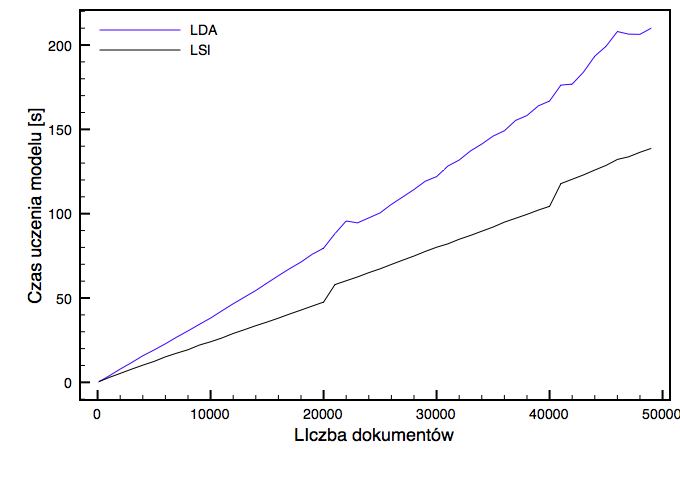
\includegraphics[width=\linewidth]{gfx/time_docs.png}
\end{figure}

\begin{figure}[h]
\caption{Czas uczenia modelu dla 5000 dokumentów}
\label{time-topics}
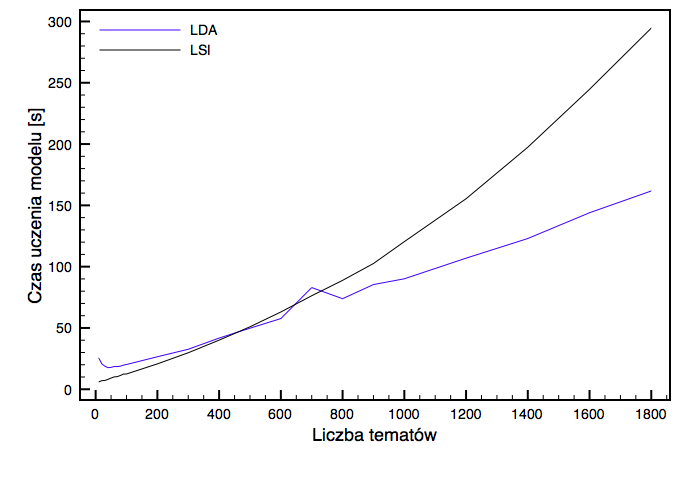
\includegraphics[width=\linewidth]{gfx/time_topics.png}
\end{figure}

\todo{Complexity discussion}
\todo{Conclusions}

\FloatBarrier

\subsection{Metryki z nadzorem}

W tym rozdziale omówiono wyniki otrzymane za pomocą algorytmów LDA i LSI dla
przykładowego problemu opisanego w \ref{sec:example}. Należy zauważyć, że tego
rodzaju ewaluacja wymaga ręcznego przygotowania danych testowych przez
człowieka, co może być nieprakyczne dla dużych zbiorów danych.  Jej zaletą jest
fakt, że mierzy ona faktyczne osiągi danego rozwiązania w rzeczywistych
problemach.

\subsubsection{Ranking dokumentów}

Wykresy \ref{ranks_stemming_comparison} i \ref{ranks_no_stemming_comparison}
przedstawiają sumę kwadratów ranków dokumentów (patrz \ref{sec:ranking}) z
wzorca przygotowanego ręcznie dla danego zapytania w wynikach działania
odpowiednio algorytmów LDA i LSI dla różnej liczby tematów.

Algorytm LDA osiąga ogólnie gorsze wyniki niż LSI - poza przedziałem $50 - 100$
tematów. Gorszy jest też (aczkolwiek niewiele) najlepszy wynik jaki udałoby się
osiągnąć odpowiednio dobierając liczbę tematów. Na wykresie daje się także
zauważyć stochastyczna natura LDA - podczas gdy dla LSI wyniki niemal
monotonicznie poprawiają się wraz ze wzrostem liczby tematów dla LDA zdarza się
znaczne pogorszenie wyników przy zwiększeniu tej liczby.

Polepszenie wyników dzięki zastosowaniu stemmingu jest widoczne na pierwszy
rzut oka --- polski jako język silnie fleksyjny jest znakomitym kandydatem do
zastosowania tego typu techniki. W \cite{manning-schuetze} zasugerowano, że ze
stemmingu można zrezygnować dyponując odpowiednio dużym zbiorem danych jednak
wyniki te uzyskano dla języka angielskiego, którego fleksja jest znacznie mniej
rozbudowana. W tym wypadku zebranie tak dużej ilości danych może być mniej
praktyczne niż skonstruowanie słownika fleksyjnego takiego jak na przykład ten
opisany w \cite{lubaszewski-slownik}.

Co ciekawe algorytm LDA radzi sobie znacznie lepiej od LSI bez wykorzystania
stemmingu.  Może to być spowodowane trudnością w przypadku LSI połączenia ze
sobą słów, które różnią się formą fleksyjną i są w tym wypadku traktownae
całkowicie osobno.

\begin{figure}[h]
\caption{Suma kwadratów ranków dokumentów ze wzorca dla testowego zapytania (z wykorzystaniem stemmingu)}
\label{ranks_stemming_comparison}
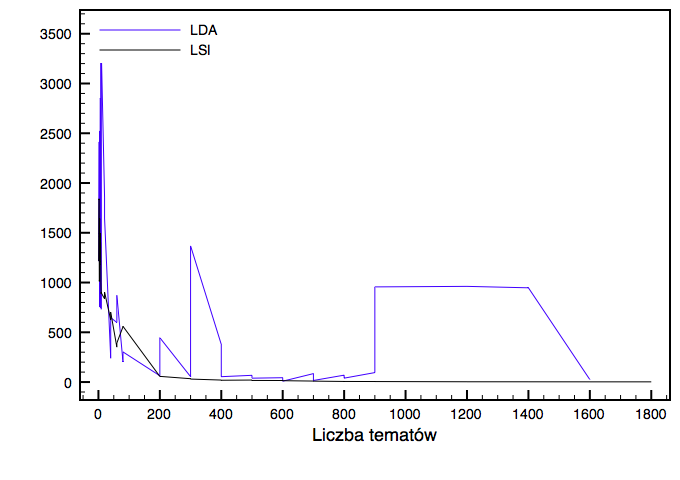
\includegraphics[width=\linewidth]{gfx/ranks_stemming.png}

\caption{Suma kwadratów ranków dokumentów ze wzorca dla testowego zapytania (bez wykorzystania stemmingu)}
\label{ranks_no_stemming_comparison}
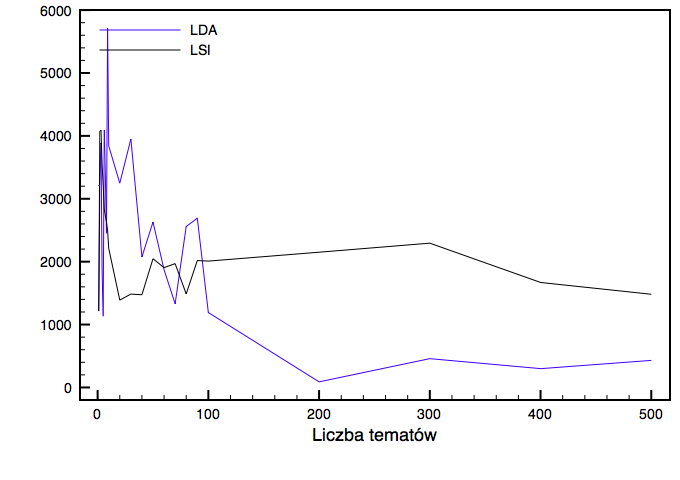
\includegraphics[width=\linewidth]{gfx/ranks_no_stemming.png}
\end{figure}

\FloatBarrier

\subsubsection{Krzywe ROC}

Krzywa ROC \cite{roc-article1} (Receiver Operation Characteristic) to wykres
przedstawiający dla danego klasyfikatora zależność między stosunkiem liczby
znalezionych dokumentów skojarzonych do liczby wszystkich zwróconych dokumentów
(TPR --- True Positive Rate), a stosunkiem liczby odrzuconych dokumentów
skojarzonych do liczby wszystkich odrzuconych dokumentów (FPR - False Positive
Rate) w miarę zmiany progu detekcji. Obliczanie tych wartości podsumowując
wzory \ref{tpr} i \ref{fpr}.

W tym wypadku ten zmienny próg to po prostu liczba $n$ - pierwszych $n$
dokumentów jest traktowane jako odnalezione, a pozostałe jako odrzucone.

\begin{equation}
\label{tpr}
TPR = \frac{TP}{TP + FN}
\end{equation}

\begin{equation}
\label{fpr}
FPR = \frac{FP}{FP + TN}
\end{equation}

Lepsze klasyfikatory charakteryzują się krzywymi ROC położonymi dalej od linii
$x = y$.  Klasyfikatory blisko, lub na tej linii nie wykonują żadnej użytecznej
pracy. Analiza odległości krzywej ROC od linii $x = y$ w różnych miejscach
wykresu może dać wskazówkę co do najlepszego dobrania progu detekcji dla danego
problemu.

Wykresy \ref{roc_lsi} i \ref{roc_lda} przedstawiają krzywe ROC dla algorytmów
LDA i LSI dla różnych liczb tematów. Dla dużych liczb tematów algorytm LDA
spisuje się gorzej, jednak można zauważyć, że klasyfikator uzyskany dla 30
tematów jest podobnej jakości lub lepszy jak ten uzyskany przy użyciu LSI dla
100 tematów.

\begin{figure}[h]
\caption{Krzywe ROC dla algorytmu LSI dla wybranych liczb tematów}
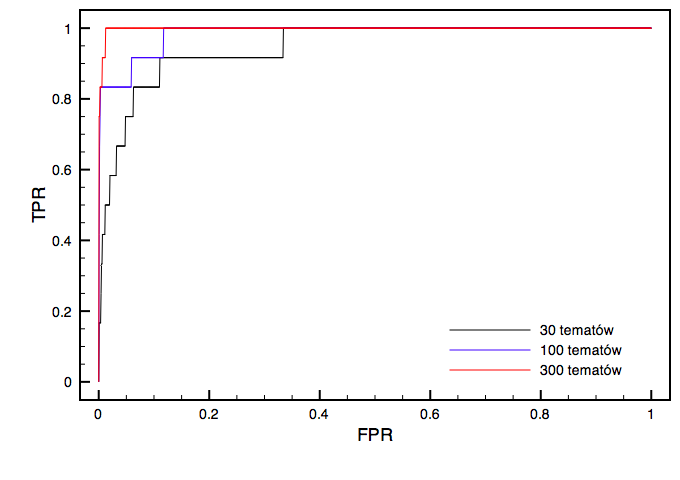
\includegraphics[width=\linewidth]{gfx/lsi_roc.png}
\label{roc_lsi}

\caption{Krzywe ROC dla algorytmu LDA dla wybranych liczb tematów}
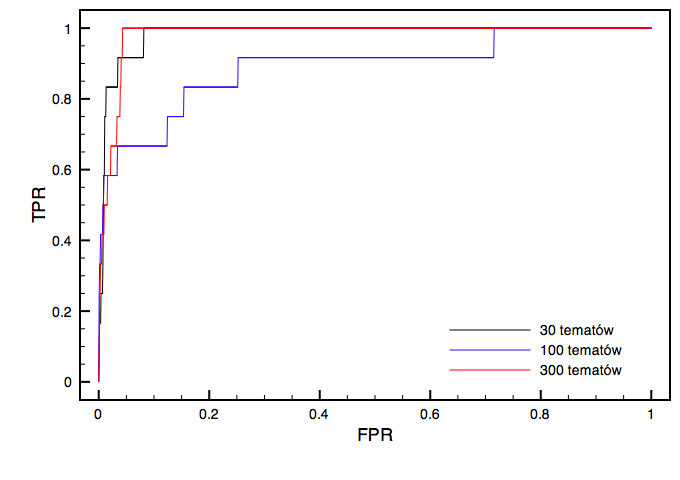
\includegraphics[width=\linewidth]{gfx/lda_roc.png}
\label{roc_lda}
\end{figure}

Na wykresach \ref{roc_lsi_untagged} i \ref{roc_lda_untagged} przedstawione
zostały krzywe ROC dla algorytmów LSI i LDA bez wykorzystania stemmingu.
Ponownie daje się zauważyć lepsze działanie algorytmu LDA w tym wypadku -
klasyfikator uzyskany dla 300 tematów jest znacznie lepszy od tego uzyskanego
przy pomocy LSI.

\begin{figure}[h]
\caption{Krzywe ROC dla algorytmu LSI dla wybranych liczb tematów bez wykorzystania stemmingu}
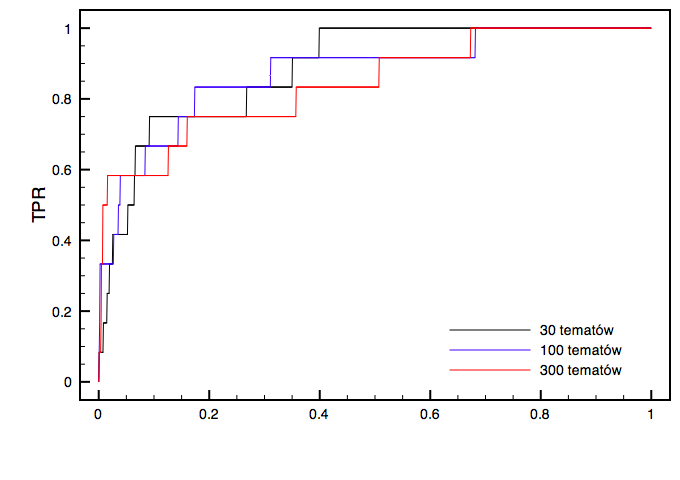
\includegraphics[width=\linewidth]{gfx/lsi_roc_untagged.png}
\label{roc_lsi_untagged}

\caption{Krzywe ROC dla algorytmu LDA dla wybranych liczb tematów bez wykorzystania stemmingu}
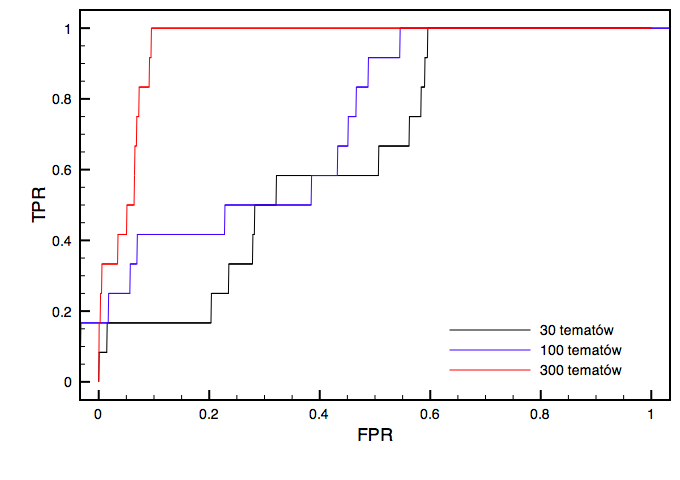
\includegraphics[width=\linewidth]{gfx/lda_roc_untagged.png}
\label{roc_lda_untagged}
\end{figure}

\FloatBarrier

\subsubsection{Dokładność i kompletność}

Kompletność (stosunek liczby zwróconych skojarzonych dokumentów do liczby
wszystkich skojarzonych dokumentów) i dokładność (stosunek liczby zwróconych
skojarzonych dokumentów do liczby wszystkich zwróconych dokumentów) to częste
metryki w zadaniach typu information retrieval. Wybranie jakiegoś poziomu
kompletności reprezentuje pewien kompromis między prawdopodobieństwem zawarcia
wszystkich interesujących wyników w zwróconych danych, a częstością
występowania w nich danych skojarzonych, a więc ilością czasu, który musi
poświęcić operator systemu na ich dalsze przetworzenie.

Wykresy \ref{fig:lsi_precision} i \ref{fig:lda_precision} prezentują dkoładność
osiąganą przez algorytmy LDA i LSI na różnych poziomach kompletności dla
przykładowego problemu.

Można zauważyć, że LDA daje znacznie gorszą dokładność niż LSI. Nawet najlepiej
dobrana liczba tematów (w tym wypadku 300) pozwala osiągać dokładność
porównywalną jedynie z LSI dla 30 tematów.

\begin{figure}[h]
\caption{Dokładność na różnych poziomach kompletności dla algorytmu LSI}
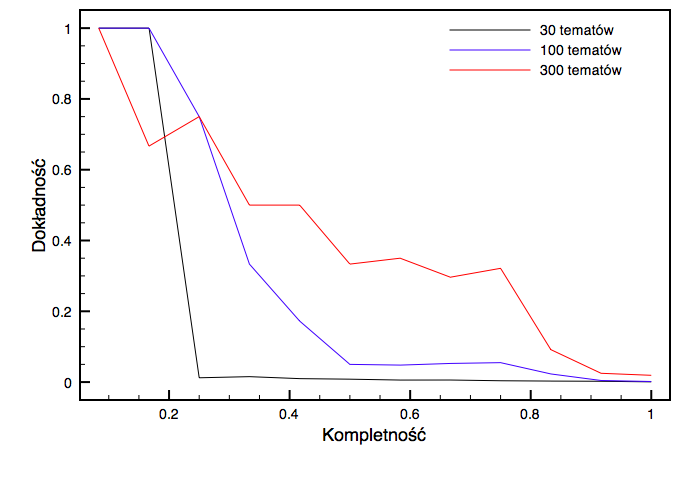
\includegraphics[width=\linewidth]{gfx/lsi_precision.png}
\label{fig:lsi_precision}
\end{figure}

\begin{figure}[h]
\caption{Dokładność na różnych poziomach kompletności dla algorytmu LDA}
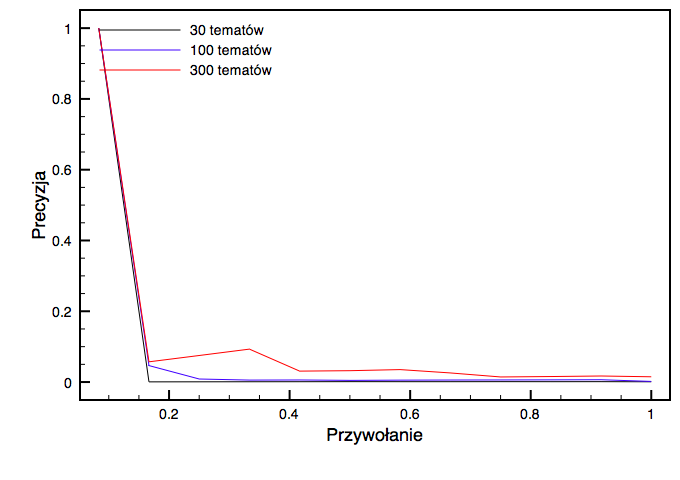
\includegraphics[width=\linewidth]{gfx/lda_precision.png}
\label{fig:lda_precision}
\end{figure}

\FloatBarrier

\subsection{Metryki bez nadzoru (perplexity)}

Współczynnik perplexity, który dla pewnych prawdopodobieństw $p_i$
przypisywanych przez model zdarzeniom obliczyć można zgodnie ze wzorem
\ref{perplexity2}, daje pewne pojęcie o tym jak dobrze model jest w stanie
przewidzieć nowe dane. Wysokie wartości współczynnika mogą wskazywać, że model
jest przeuczony i będze słabo uogólniał swoje działania na nieznane dane. Jest
on dobrym wskaźnikiem jak dobrze model będzie sobie radził z klastrowaniem tego
typu danych.

\begin{equation}
  \label{perplexity2}
  \frac{2^{-\sum_{i/1}^n p_ilog_2(p_i)}}{n}
\end{equation}

Wartości współczynnika perplexity dla omawianych metod w zależności od liczby
tematów są przedstawione na wykresie \ref{fig:perplexity}, Wykres demonstruje,
że optymalne wartości współczynnika perplexity zostają osiągnięte w okolicach
50 tematów. W tym wypadku może to sugerować, że mniej więcej na tyle właśnie
grup tematycznych należałoby podzielić ten zbiór danych.

Algorytm LDA zachowuje niski współczynnik perplexity tylko stosunkowo blisko
optymalnej liczby tematów. Takie zachowanie może wymagać dokładnego strojenia
algorytmu do każdego zastosowania, co bywa uciążliwe i czasochłonne.

\begin{figure}[h]
\caption{Współczynnik perplexity dla LDA i LSI w zależności od liczby tematów}
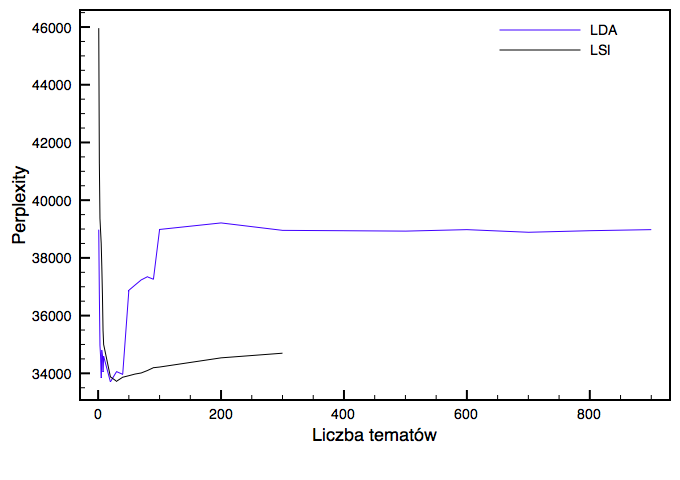
\includegraphics[width=\linewidth]{gfx/perplexity.png}
\label{fig:perplexity}
\end{figure}

\FloatBarrier

\subsection{Wnioski}

Algorytm LDA daje gorszej jakości (a przynajmniej mniej stabilne) wyniki dla
typowych problemów klasyfikacji i wyszukiwania informacji spotykanych w
codziennej praktyce. Wydaje się za to być w stanie działać w sytuacji, gdy
wiele różnych tokenów oznacza to samo (przypadek bez wykorzystania stemmingu),
w odróżnieniu od LSI, którego wyniki są wtedy całkowicie nieprzydatne. To
bardzo porządana cecha w przypadku braku odpowiedniego słownika fleksyjnego dla
danego języka.

Przewagą LDA wydaje się być jakość generowanych tematów --- przez wymuszenie
dodatnich wag otrzymujemy na najbardziej znaczących pozycjach (z najwyższymi
wagami) słowa opisujące dany dokument/temat, podczas gdy w przypadku LSI mogą
to być słowa najodleglejsze. Takie zachowanie może okazać się korzystne w
zastosowaniach typu tagowanie dokumentów lub automatyczne generowanie
podsumowań czy słów kluczowych.

\section{Podsumowanie}

\appendix
\section{Sposób użycia kodu}

Kod wykorzystany do przeprowadzenia badań w tej pracy znaleźć można pod
\cite{code}. Aby z niego skorzystać konieczne jest zainstalowanie pakietu
gensim. Katalog \emph{bin} zawiera skrypty uruchomieniowe dla przeprowadzonych
eksperymentów. W poniżych poleceniach \emph{model} oznaczna ciąg
\emph{LsiModel} lub ciąg \emph{LdaModel} w zależności od rodzaju modelu, który
ma być testowany. Plik z danymi powinien zawierać dokumenty, każdy w jednej
linii, wyrazy powinny być sprowadzone do form podstawowych, jeżeli takie
rozwiązanie ma być zastosowane.

\begin{itemize}
\item \emph{bin/test\_lsi [plik z korpusem] [model]} --- wypisuje na ekran
listę wygenerowanych tematów
\item \emph{bin/map\_topics [plik z korpusem] [model]} --- oblicza i wypisuje
metrykę $M$ dla różnych liczb tematów
\item \emph{bin/perplexity [plik z korpusem] [model]} --- oblicza i wypisuje
współczynnik perplexity dla różnych liczb tematów
\item \emph{bin/precision [plik z korpusem] [model] [liczba tematów]} ---
oblicza i wypisuje zależność między dokładnością a kompletnością w formie
par [dokładność kompletność] dla zadanej liczby tematów
\item \emph{bin/roc [plik z korpusem] [model] [liczba tematów]} ---
oblicza i wypisuje zależność między TPR a FPR w formie
par [TPR FPR] dla zadanej liczby tematów
\end{itemize}

\addcontentsline{toc}{section}{Spis tablic}
\listoftables
\addcontentsline{toc}{section}{Spis rysunków}
\listoffigures
\addcontentsline{toc}{section}{Literatura}
\bibliographystyle{abbrv}
\bibliography{thesis}

\enddocument
